\documentclass[12pt,a4paper,twoside]{report}         
\usepackage{cs}              
\usepackage{times}
\usepackage{graphicx}
\usepackage{latexsym}
\usepackage{amsmath,amsbsy}
\usepackage{amssymb}
\usepackage[matrix,arrow]{xy}
\usepackage[T1]{fontenc}
\usepackage{ae,aecompl}
%\usepackage{shortcut} %definitii pentru diacritice; 
\usepackage{amstext}
\usepackage{graphics}
\usepackage[T1]{fontenc}
\usepackage{ae,aecompl}
\usepackage{algorithm}
%\usepackage{algorithmic}
\usepackage{color}
\usepackage{color}
\usepackage{wrapfig}
\usepackage{subcaption}
\usepackage{array}
\usepackage[table]{xcolor}

% \mastersthesis
\diplomathesis
% \leftchapter
\centerchapter
% \rightchapter
\singlespace
% \oneandhalfspace
% \doublespace

\renewcommand{\thesisauthor}{Radu PETRIŞEL}    %% Your name.
\renewcommand{\thesismonth}{June}     %% Your month of graduation.
\renewcommand{\thesisyear}{2019}      %% Your year of graduation.
\renewcommand{\thesistitle}{REACTIVE PROGRAMMING BASED GESTURE DETECTION IN VIRTUAL REALITY USING LEAPMOTION} 
\renewcommand{\thesissupervisor}{Assist. Prof. Dr. Eng. Adrian SABOU}
\newcommand{\department}{\bf FACULTY OF AUTOMATION AND COMPUTER SCIENCE\\
COMPUTER SCIENCE DEPARTMENT}
\newcommand{\thesis}{LICENSE THESIS}
\newcommand{\utcnlogo}{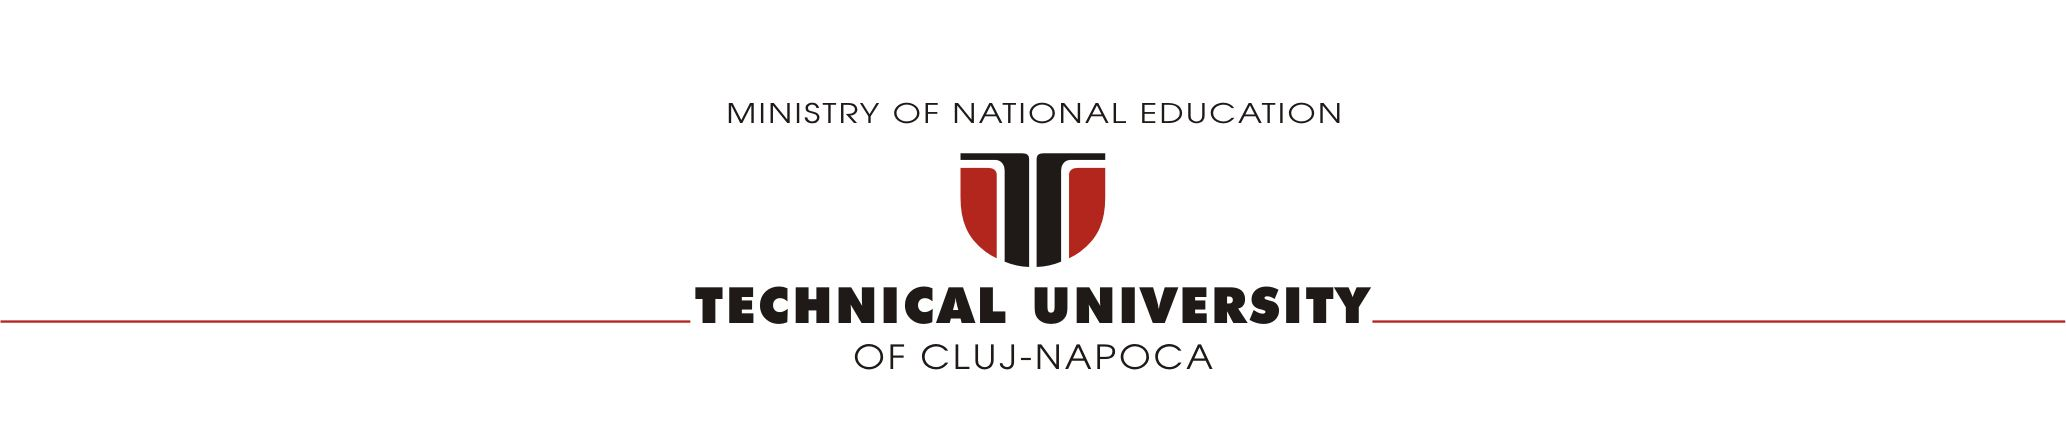
\includegraphics[width=15cm]{img/tucn.jpg}}

\newcommand{\uline}[1]{\rule[0pt]{#1}{0.4pt}}
%\renewcommand{\thesisdedication}{P\u{a}rin\c{t}ilor mei}

\begin{document}
%\frontmatter
%\pagestyle{headings}

\newenvironment{definition}[1][Defini\c{t}ie.]{\begin{trivlist}
\item[\hskip \labelsep {\bfseries #1}]}{\end{trivlist}}

%\thesistitle                    %% Generate the title page.
%\authordeclarationpage                %% Generate the declaration page.

\setcounter{secnumdepth}{3}

\pagenumbering{Roman}
\setcounter{page}{1}

\begin{center}
\utcnlogo

\department

\vspace{4cm}

{\bf \thesistitle} %LICENSE THESIS TITLE}

\vspace{1.5cm}

\thesis
\vspace{5.75cm}

Graduate: {\bf \thesisauthor{}} 

Supervisor: {\bf \thesissupervisor{}}

\vspace{3cm}
{\bf \thesisyear}
\end{center}

\thispagestyle{empty}
\newpage

\begin{center}
\utcnlogo

\department

\end{center}
\vspace{0.5cm}

%\begin{small}
\begin{tabular}{p{7cm}p{8cm}}
 %\hspace{-1cm}& APPROVED,\\
 \hspace{-1cm}DEAN, & HEAD OF DEPARTMENT,\\
 \hspace{-1cm}{\bf Prof. dr. eng. Liviu MICLEA} & {\bf Prof. dr. eng. Rodica POTOLEA}\\  
\end{tabular}
 
\vspace{2cm}

\begin{center}
Graduate: {\bf \thesisauthor}

\vspace{1cm}

{\bf \thesistitle}
\end{center}

\vspace{1cm}

\begin{enumerate}
  \item {\bf Project proposal:} {\it A Reactive Programming oriented Unity asset for gesture detection using the LeapMotion controller}
  \item {\bf Project contents:} {\it (enumerate the main component parts) Presentation page, advisor's evaluation, title of chapter 1, title of chapter 2, ..., title of chapter n, bibliography, appendices.}
  \item {\bf Place of documentation:} {\it Technical University of Cluj-Napoca, Computer Science Department}
  \item {\bf Consultants:} \thesissupervisor{}
  \item {\bf Date of issue of the proposal:} November 1, 2018
  \item {\bf Date of  delivery:} June 14, 2019
\end{enumerate}

\vspace{1.2cm}

\hspace{6cm} Graduate: \uline{6cm} 

\vspace{0.5cm}
\hspace{6cm} Supervisor: \uline{6cm} 
%\end{small}

\thispagestyle{empty}


\newpage
$ $
%\begin{center}
%\utcnlogo

%\department
%\end{center}

\thispagestyle{empty}
\newpage

\begin{center}
\utcnlogo

\department
\end{center}

\vspace{0.5cm}

\begin{center}
{\bf
Declara\c{t}ie pe proprie r\u{a}spundere privind\\ 
autenticitatea lucr\u{a}rii de licen\c{t}\u{a}}
\end{center}
\vspace{1cm}



Subsemnatul(a) \\
\uline{14.8cm}, 
legitimat(\u{a}) cu \uline{4cm} seria \uline{3cm} nr. \uline{4cm}\\
CNP \uline{9cm}, autorul lucr\u{a}rii \uline{2.8cm}\\
\uline{16cm}\\
\uline{16cm}\\
elaborat\u{a} \^{\i}n vederea sus\c{t}inerii examenului de finalizare a studiilor de licen\c{t}\u{a} la Facultatea de Automatic\u{a} \c{s}i Calculatoare, Specializarea \uline{7cm} din cadrul Universit\u{a}\c{t}ii Tehnice din Cluj-Napoca, sesiunea \uline{4cm} a anului universitar \uline{3cm}, declar pe proprie r\u{a}spundere, c\u{a} aceast\u{a} lucrare este rezultatul propriei activit\u{a}\c{t}i intelectuale, pe baza cercet\u{a}rilor mele \c{s}i pe baza informa\c{t}iilor ob\c{t}inute din surse care au fost citate, \^{\i}n textul lucr\u{a}rii \c{s}i \^{\i}n bibliografie.

Declar, c\u{a} aceast\u{a} lucrare nu con\c{t}ine por\c{t}iuni plagiate, iar sursele bibliografice au fost folosite cu 
respectarea legisla\c{t}iei rom\^{a}ne \c{s}i a conven\c{t}iilor interna\c{t}ionale privind drepturile de autor.

Declar, de asemenea, c\u{a} aceast\u{a} lucrare nu a mai fost prezentat\u{a} \^{\i}n fa\c{t}a unei alte comisii de examen de licen\c{t}\u{a}.

\^{I}n cazul constat\u{a}rii ulterioare a unor declara\c{t}ii false, voi suporta sanc\c{t}iunile administrative, respectiv, \emph{anularea examenului de licen\c{t}\u{a}}.

\vspace{1.5cm}

Data \hspace{8cm} Nume, Prenume

\vspace{0.5cm}

\uline{3cm} \hspace{5cm} \uline{5cm}

\vspace{0.5cm}
\hspace{9.4cm}Semn\u{a}tura

\thispagestyle{empty}

\newpage

\tableofcontents
\newpage

\pagenumbering{arabic}
\setcounter{page}{1}


\chapter{Introduction - Project Context}
\pagestyle{headings}

Virtual Reality is an experience that has gained huge popularity in the recent years. Because of this new means of interaction with this virtual world are needed and they should feel as natural as possible. Ergo, hand tracking and gesture detection is a "must have" for modern VR applications.

\section{Virtual reality}
The term "virtual" began its life in the late 1400s, meaning "being something in essence or effect, though not actually or in fact" \cite{Virtual}, but, in the IT context, the word has the meaning "not physically existing but made to appear by software" \cite{Virtual}. The original use of the phrase "virtual reality" is found in French playwright' Antonin Artaud collection of essays \textit{Le Théâtre et son double}, first published in 1938 \cite{TheatreAndItsDouble}.

\subsection{History}
The precise roots of virtual reality are challenged, partially because of how hard it was to formulate a definition of an alternate reality notion. In 1968, Ivan Sutherland created what was widely regarded as the first head-mounted display system for use in immersive simulation applications, with the help of his students. In the next two decades, VR devices were mainly used for medical, automobile industry design, militry training and flight simulation purposes.

The 1990s saw the first commercially extensive release of consumer headsets, notably \textit{Sega VR} (1991) and \textit{Sega VR-1} (1994) launched by Sega, and \textit{Nintendo's Virtual Boy} (1995). The 2000s were a period of comparative indifference from the public and investment towards VR techniques available on the market. Google launched \textit{Street View} in 2007, a service that offers panoramic views of a growing amount of global locations such as highways, indoor houses and rural regions, which also integrates a stereoscopic 3D mode as of 2010.

The modern, consumer version of headsets started developing in the early 2010s. In 2013, Valve Corporation found and freely shared the breakthrough of low-persistence screens that make it possible today to show VR content lag-free and smear-free. 

\begin{wrapfigure}[16]{r}{0.25\textwidth}
  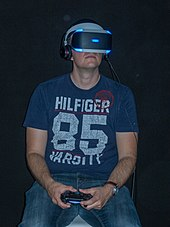
\includegraphics[width=1.1\linewidth]{img/Sony_morpheus.jpg}
  \caption{Project Morpheus (PlayStation VR) at gamescom in 2015}
  \label{fig:morpheus}
\end{wrapfigure}

This discovery was quickly adopted by the other companies on the market, with Sony announcing \textit{Project Morpheus} in 2014 and Google announcing \textit{Cardboard} in 2015. In 2016, HTC released and shipped the first units of \textit{Vive SteamVR}, the first major commercial headset for average users.

\subsection{Modern technology}

Present virtual reality headset displays rely on smartphone technologies including: gyroscopes and motion sensors for head, hand and body position monitoring, tiny high definition stereoscopic displays and small, lightweight and powerful computer processors.

Special input devices are required for interaction with the virtual world, such as hand controllers, haptic gloves, 3D mouse and optical tracking sensors. Both haptic gloves and hand controllers provide force feedback (in the form of vibration), with haptic gloves providing also feedback in the form of response force (like when picking a rubber duck).

\section{Gesture recognition}

\begin{wrapfigure}[14]{l}{0.45\linewidth}
  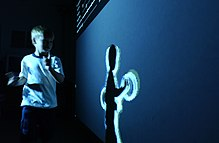
\includegraphics[width=\linewidth]{img/GestRecog_child.jpg}
  \caption{A child being recognized by a simple gesture detection algorithm}
  \label{fig:child}
\end{wrapfigure}

Gesture recognition is an active research field with the objective of comprehending human gestures through mathematical models. Gestures can come from any posture or position of the body, but they typically come from the hand. Without actually touching them, users can use simple motions to command or communicate with machines.

Gesture recognition may be seen as a means for machines to commence to comprehend human body language, establishing a stronger link between computers and individuals than conventional text user interfaces or even GUIs (graphical user interfaces), which still restrict most inputs to the keyboard and/or mouse and communicate naturally with no mechanical instruments.

\section{Reactive programming}
Reactive programming is a declarative programming paradigm concerned with asynchronous data streams and the propagation of change. With this paradigm it is feasible to easily express static (e.g. lists) or dynamic (e.g. events) information streams and to also indicate that an implied dependency remains within the related implementation model, which promotes the automatic propagation of the altered information stream.

Examples of Reactive Programming include hardware description languages (HDLs), such as VHDL or Verilog, in which changes are modeled as they propagate through a circuit. As a manner to optimize the development of dynamic user interfaces and virtually-real-time system animation, reactive programming has been suggested.

\chapter{Project Objectives and Specifications}

\section{Introduction}
The purpose of this chapter is to collect, analyze and define high-level needs and features of the Unity asset named Fluent Motion. It focuses on the capabilities needed by the stakeholders and the target users, and why these needs exist.

\section{Positioning}
\subsection{Problem statement}

As Virtual Reality (VR) is becoming more accessible to the average person, more problems arise with the means of interacting with the VR world. A solution to this issue is the Leap Motion hand tracking device, which offers a natural means of human-VR interaction. The problem with Leap Motion is its non-friendly Application Programmer Interface (API). 

\newcolumntype{g}{>{\columncolor{lightgray}} m{0.45\linewidth}}

\begin{table}[h]
  \centering
  \begin{tabular}{| g | m{0.45\linewidth} |}
    \hline
    \textbf{The problem of} & Leap Motion’s unfriendly API \\
    \hline
    \textbf{affects} & developers in the VR field who use Leap Motion \\
    \hline
    \textbf{the impact of which is} & a limited number of applications using Leap Motion \\
    \hline
    \textbf{a successful solution would be} & 
      easy to use

      fluent (in terms of code readability)

      adhere to the reactive programming paradigm

      available on Unity's asset store
      \\
    \hline
  \end{tabular}
  \label{table:problem_statement}
\end{table}

\subsection{Product Position Statement}
Fluent Motion comes as a union between three technologies – Virtual Reality, Leap Motion and ReactiveX.

So far, Virtual Reality and Leap Motion already are integrated (by means of LeapMotion’s API), but ReactiveX can offer a more fluent way of expressing what an application using the first two mentioned technologies together. 

\begin{table}[h]
  \centering
  \begin{tabular}{| g | m{0.45\linewidth} |}
    \hline
    \textbf{For} & Virtual Reality developers \\
    \hline
    \textbf{who} & use Leap Motion \\
    \hline
    \textbf{Fluent Motion} & is an extension of Leap Motion using ReactiveX \\
    \hline
    \textbf{that} & offers a fluent API for Leap Motion \\
    \hline
    \textbf{unlike} & the default API \\
    \hline
    \textbf{Fluent Motion will} &
      be easy to use    
      
      be fluent (in terms of code readability)

      adhere to the reactive programming paradigm \\
    \hline
  \end{tabular}
  \label{table:problem_statement}
\end{table}

\section{Stakeholder and User Descriptions}

\subsection{Stakeholder summary}

\begin{table}[h]
  \centering
  \begin{tabular}{| m{0.3\linewidth} | m{0.3\linewidth} | m{0.3\linewidth} |}
    \hline
    \rowcolor{lightgray} Name & Description & Responsibilities \\
    \hline
    \textbf{Developer (VR)} & Person who wants to create Virtual Reality applications & Use Fluent Motion \\
    \hline
    \textbf{Developer (Fluent Motion)} & Person who creates and maintains Fluent Motion & Create, improve and offer technical support for Fluent Motion \\
    \hline
  \end{tabular}
\end{table}

\subsection{User summary}

\begin{table}[h]
  \centering
  \begin{tabular}{| m{0.22\linewidth} | m{0.22\linewidth} | m{0.22\linewidth} | m{0.22\linewidth} |}
    \hline
    \rowcolor{lightgray} Name & Description & Responsibilities & Stakeholder \\
    \hline
    \textbf{Developer (VR)} & Person who wants to create VR applications & Use Fluent Motion & \textit{Developer (VR)} \\
    \hline
  \end{tabular}
\end{table}

\subsection{User environment}

\subsubsection{Users}
The API will be used by developer teams of any size.

\subsubsection{Infrastructure}
The infrastructure needed by Fluent Leap is an aggregation of the hardware requirements of the combined systems and technologies, i.e.:

\begin{table}[h]
  \centering
  \begin{tabular}{| m{0.2\linewidth} | m{0.7\linewidth} |}
    \hline
    Operating system & \textbf{Windows 7 SP1}, \textbf{Windows 8.1} or later, \textbf{Windows 10} \\
    \hline
    Middleware & \textbf{SteamVR} platform \\
    \hline
    Additional 
    
    hardware & \textbf{Leap Motion} hand tracking device

    a VR headset (at the time of writing, \textbf{Occulust Rift}, \textbf{HTC Vive} or \textbf{Valve Index}) \\
    \hline
    Miscellaneous & \textbf{.NET Framework 4.6} or newer

    \textbf{Unity} 5.6 or later \\
    \hline
  \end{tabular}
\end{table}

\subsection{Summary of key stakeholder or user needs}

\begin{table}[h]
  \centering
  \begin{tabular}{| m{0.18\linewidth} | m{0.08\linewidth} | m{0.18\linewidth} | m{0.26\linewidth} | m{0.21\linewidth} | }
    \hline
    \rowcolor{lightgray} Need & Priority & Concerns & Current solution & Proposed solution \\
    \hline
    \textbf{VR API} & 0 & Developer & Leap Motion default API, using \textbf{ANSI C} language imperative style & Fluent Motion, using \textbf{C\#} language and ReactiveX \\
    \hline
    \textbf{Desktop API} & 1 & Developer & Leap Motion default API, using \textbf{ANSI C} language impertive style & Fluent Motion, using \textbf{C\#} language and ReactiveX \\
    \hline
    \textbf{Usability} & 0 & Developer & Leap Motion defualt API, using \textbf{ANSI C} language imperative style & Fluent Motion, using \textbf{C\#} language and ReactiveX \\
    \hline
  \end{tabular}
\end{table}

\subsection{Alternatives and competetion}
External competition is represented by the current API offered by LeapMotion.

\section{Product overview}
\begin{wrapfigure}[10]{r}{0.3\linewidth}
  \centering
  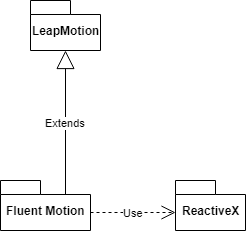
\includegraphics[width=\linewidth]{img/Product_arch.png}
  \caption{Fluent Motion architectural diagram}
  \label{fig:arch}
\end{wrapfigure}

The API should provide all the functionality already provided by Leap Motion's default API, but in a higher-level language.

\subsection{Product perspective}
This product will extend existing features from Leap Motion, making them more readable and developer friendly.

\subsection{Assumption and dependencies}
For developers:
\begin{table}[h]
  \centering
  \begin{tabular}{| m{0.2\linewidth} | m{0.7\linewidth} |}
    \hline
    Operating system & \textbf{Windows 7 SP1}, \textbf{Windows 8.1} or later, \textbf{Windows 10} \\
    \hline
    Middleware & \textbf{SteamVR} platform \\
    \hline
    Additional 
    
    hardware & \textbf{Leap Motion} hand tracking device

    a VR headset (at the time of writing, \textbf{Occulust Rift}, \textbf{HTC Vive} or \textbf{Valve Index}) \\
    \hline
    Miscellaneous & \textbf{.NET Framework 4.6} or newer

    \textbf{Unity} 5.6 or later \\
    \hline
  \end{tabular}
\end{table}

For end products that reference Fluent Motion:

\begin{table}[h]
  \centering
  \begin{tabular}{| m{0.2\linewidth} | m{0.35\linewidth} | m{0.35\linewidth} |}
    \hline
    \rowcolor{lightgray} & Minimum & Recommended \\
    \hline
    \textbf{CPU} & Intel Core i3-8100 & Intel i5-4590 or AMD FX 8350 equivalent \\
    \hline
    \textbf{GPU} & Nvidia GeForce GTX 1060 3GB or AMD Radeon RX 570 & Nvidia GeForce GTX 970 or AMD Radeon R9 290 equivalent \\
    \hline
    \textbf{Memory} & 8GB & 16GB \\
    \hline
    \textbf{Output} & HDMI 1.4, DisplayPort 1.2 & DisplayPort 1.2 \\
    \hline
    \textbf{Input} & 2x USB 3.1 gen 1 (Type-A) & 2x USB 3.1 gen 2 (Type-A) \\
    \hline    
  \end{tabular}
\end{table}

\section{Product features}
\begin{enumerate}
  \item \textbf{Hands module}

    The module that will allow the developer to use the two hands objects from the scene in order to detect gestures or motions, and assign callbacks when certain criteria regarding the hands are met.\\
    This module is available in both Virtual Reality and Desktop modes.

  \item \textbf{Fingers module}

    The module that will allow the developer to use the fingers (individually or in groups) in the scene for detecting gestures or motions, and assign callbacks when certain criteria regarding the fingers are met.\\
    This module is available in both Virtual Reality and Desktop modes.

  \item \textbf{Virtual Reality module}

    The module that will allow the user to develop Virtual Reality applications.   This module will act as a dependency to other modules. \\
    It isn’t mutually exclusive with the Desktop Module, BUT at least one of the two must be present.

  \item \textbf{Desktop module}

    The module that will allow the user to develop applications using Leap Motion in desktop mode.\\
    This module will act as dependency to other modules. It isn’t mutually exclusive with the Virtual Reality Module, BUT at least one of the two must be present.
  
  \item \textbf{Gesture definition module}
    
    The module that allows the user to define new gestures besides already existing ones.\\
    This module depends on either Virtual Reality module or Desktop module, and on either Hands module, Fingers module or both.

  \item \textbf{Gestures module}

    This module will provide defitions to some basic gestures (like finger pointing to some object, hand swipe, etc.).
    This module depends on either Virtual Reality module or Desktop module, and on either Hands module and Fingers module.

  \item \textbf{Demo}

    This module will provide some demonstrative code for new users to acquaint themselves with the basic flows and code syntax of Fluent Motion.
  
\end{enumerate}

\section{Other product requirements}

\begin{enumerate}
  \item \textbf{High readability}
    
    The main purpose of the API is to be fluently read, i.e. the code should sound almost like natural language when read by other developers.

  \item \textbf{Open source}
  
    The project will be open source and anyone will be able to contribute to it.

  \item \textbf{Performance}

    Virtual Reality applications shouldn’t fall bellow 80 frames per second (FPS), and, as such, the API shouldn’t introduce a high processing time per frame to to fall below that threshold.

  \item \textbf{Scalability}
    
    The API should support detecting up to 10 distinct gestures per application and interacting with at least 20 objects (excluding hand to hand interactions).

  \item \textbf{Maintainability}

    The VR world is still young and technologies evolve fast, so the API should be highly maintainable to keep its edge.

  \item \textbf{Extendibility}
    
    The API should be easily extendable by any backer on Git.

\end{enumerate}

\chapter{Bibliographic research}

\section{Gestures}

\begin{wrapfigure}[20]{l}{0.4\textwidth}
  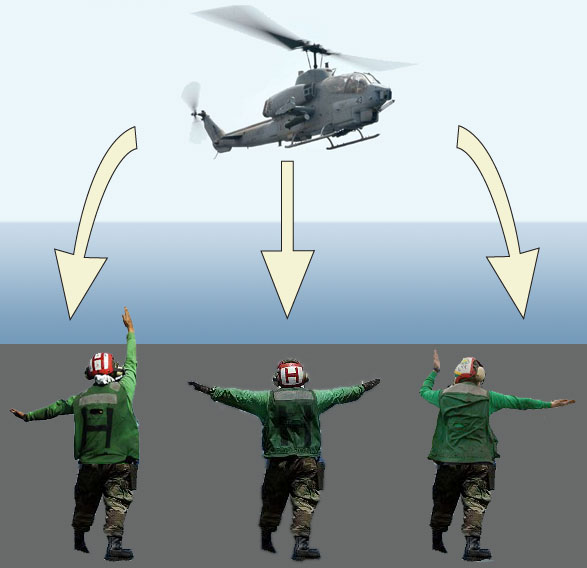
\includegraphics[width=0.9\linewidth]{img/Gesture_navy.jpg}
  \caption{Military air marshallers use hand and body gestures to direct flight operations aboard aircraft carriers}
  \label{fig:air_marshallers}
\end{wrapfigure}

A gesture is a type of non-verbal communication in which real physical movements transmit specific messages, both in place or in combination with speech. Gestures include movement of the hands, face, or other parts of the body. Gestures differ from physical non-verbal communication that does not communicate specific messages, such as purely expressive displays, proxemics, or displays of joint attention. \cite{Gestures}

Gestures can be of two types: \textit{informative (passive)} or \textit{communicative (active)}. 

\section{Leap Motion}

The \textit{Leap Motion Controller} is a tiny peripheral USB device intended to be facing upwards on a physical desktop, but can also be mounted on a VR headset.

\begin{figure}[h]
  \centering
  \begin{subfigure}{0.45\textwidth}
    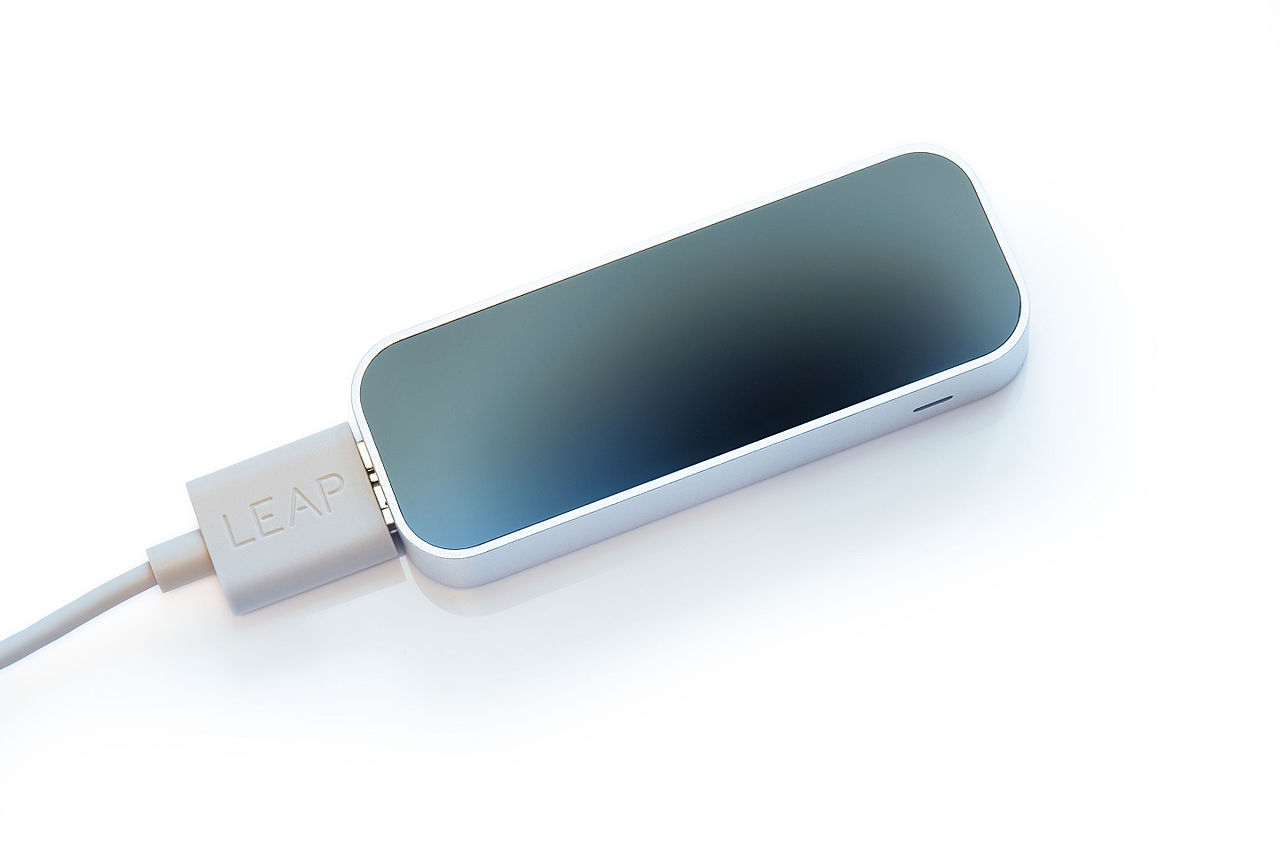
\includegraphics[width=\linewidth]{img/Leap_motion.jpg}
    \caption{The LeapMotion controller}
    \label{fig:leap_controller}
  \end{subfigure}
  \begin{subfigure}{0.45\textwidth}
    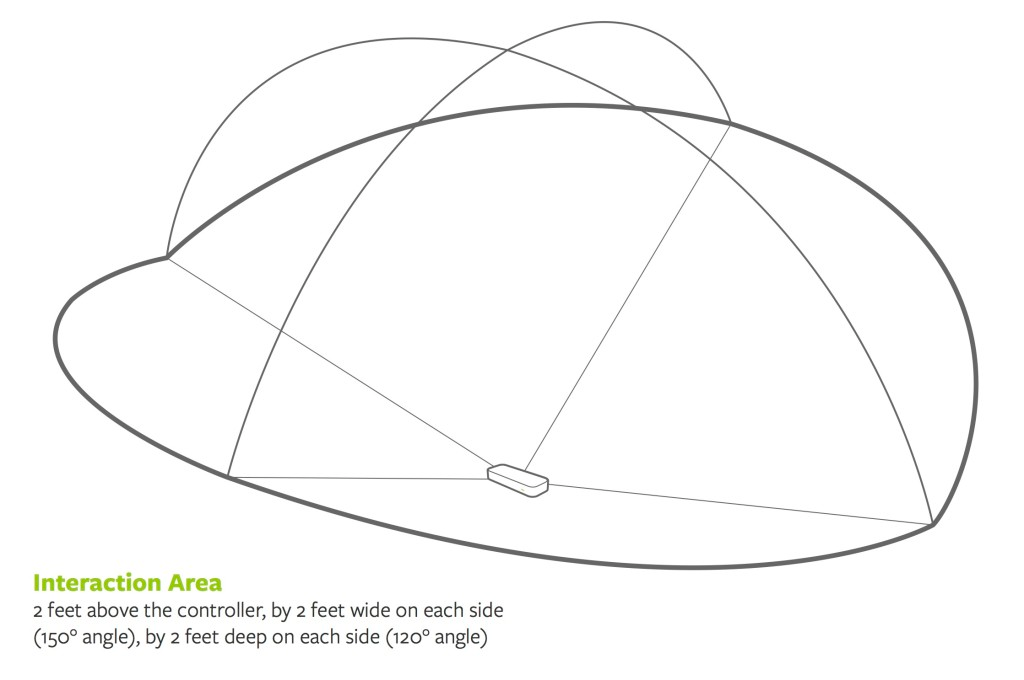
\includegraphics[width=\linewidth]{img/Leap_interaction.png}
    \caption{The interaction area}
    \label{fig:leap_interaction}
  \end{subfigure}
  \caption{The LeapMotion system}
\end{figure}

\subsection{Hardware}

The \textit{Leap Motion Controller} is really quite straightforward from a hardware view. Two cameras and three infrared LEDs are the core of the device. These track infrared light with a wavelength of 850 nanometers, which is outside the visible light spectrum. \cite{LeapArticle}

The unit has a big interaction room of 0.22 m\textsuperscript{3} thanks to its wide-angle glasses, which takes the form of an inverted pyramid – the intersection of the areas of perspective of the binocular cameras (see figure \ref{fig:leap_interaction}). The viewing range of the device is 60cm to 80cm, depending on the version of the firmware used.

This raw data is then stored in the device's local memory and then sent via USB to the \textit{Leap Motion tracking software}. As the cameras work with near-infrared light, the data is in the form of grayscale stereo images, as shown in figure \ref{fig:leap_raw}.

\begin{figure}[h]
  \centering
  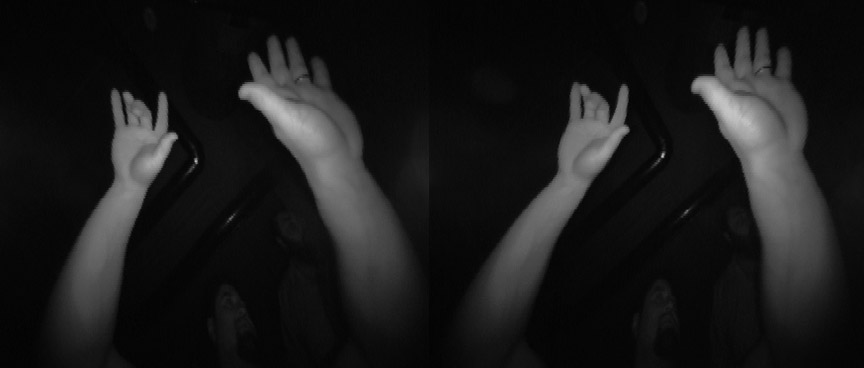
\includegraphics[width=0.9\linewidth]{img/Leap_raw.jpg}
  \caption{Leap Motion raw data}
  \label{fig:leap_raw}
\end{figure}

\subsection{Sofware}

It's time for some heavy mathematical lifting once the picture information is streamed to the computer. The \textit{Leap Motion Controller} does not produce depth maps despite common misconceptions - instead it applies sophisticated algorithms to the raw sensor information.

\begin{wrapfigure}[9]{l}{0.4\textwidth}
  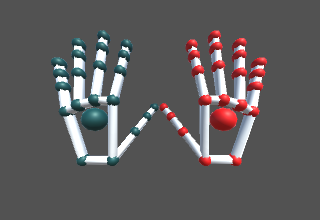
\includegraphics[width=0.37\textwidth]{img/Leap_capsule_hands.png}
  \caption{Capsule hands}
  \label{fig:leap_capsule}
\end{wrapfigure}

The Leap Motion Service first compensates background objects (e.g. head) and lightning, and then extracts from the data the relevant information - arms, hands and fingers.

Though a transport layer, the results(frames) are fed to the \textit{Leap Motion Control Panel} or to native and web clients. These orgaize the data into an object-orietented structure.

\section{Reactive Extensions}

ReactiveX is a library for composing asynchronous and event-based programs by using observable sequences. \cite{RX_intro}

It extends the observer pattern to support data and/or event sequences and provides operators that help you compose sequences declaratively while abstracting issues such as low-level threading, synchronization, thread security, concurrent data structures, and non-blocking I/O.

Table \ref{table:rx} shows how observables integrate in the programming world.

\begin{table}[h]
  \centering
  \begin{tabular}{c | c | c}
    & single items & multiple items \\
    \hline
    synchronous & T GetData & IEnumerable<T> GetData \\
    asynchronous & Awaitable<T> GetData & Observable<T> GetData
  \end{tabular}
  \caption{Observable position in multiple items and asynchronous world}
  \label{table:rx}
\end{table}

\subsection{Why use observables?}
ReactiveX observables are intended to be \textbf{\textit{composable, flexible}}and \textbf{\textit{less opitionated}}. These provide a huge advantage over structures like Java \textit{Futures} or C\# \textit{Awaitables}, because it removes the need for ambiguous nesting of callbacks.

RX Observables also offer three methods for of flow control - \textit{OnNext}, \textit{OnError} and \textit{OnCompleted} - which give the programmer very much liberty.

\begin{figure}[h]
  \centering
  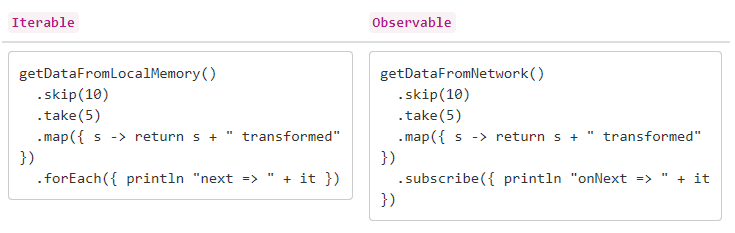
\includegraphics[width=\textwidth]{img/RX_iterable_vs_observable.PNG}
  \caption{Iterable vs Observable}
  \label{fig:rx_obs_it}
\end{figure}


% Bibliographic research has as an objective the establishment of the references for the project, within the project domain/thematic. While writing this chapter (in general the whole document), the author will consider the knowledge accumulated from several dedicated disciplines in the second semester, 4$^{th}$ year (Project Elaboration Methodology, etc.), and other disciplines that are relevant to the project theme.

% Represents about 15\% of the paper.

% Each reference must be cited within the document text, see example below (depending on the project theme, the presentation of a method/application can vary).

% This section includes citations for conferences or workshop~\cite{BellucciLZ04}, journals~\cite{AntoniouSBDB07}, 
% and books~\cite{russell1995artificial}. 

% In paper~\cite{AntoniouSBDB07} the authors present a detection system for moving obstacles based on stereovision and ego motion estimation. 
% The method is ... {\it discus the algorithms, data structures, functionality, specific aspects related to the project theme, etc.}... Discussion: {\it pros and cons}.

% In chapter~\ref{ch:analysis} of~\cite{strunk}, the {\it similar-to-my-project-theme algorithm} is presented, with the following features ...


\section{Title}
\section{Other title}


\chapter{Analysis and Theoretical Foundation}
\label{ch:analysis}

Together with the next chapter takes about 60\% of the whole paper

The purpose of this chapter is to explain the operating principles of the implemented application.
Here you write about your solution from a theory standpoint - i.e. you explain it and you demonstrate its theoretical properties/value, e.g.:
\begin{itemize}
 \item used or proposed algorithms
 \item used protocols
 \item abstract models
 \item logic explanations/arguments concerning the chosen solution
 \item logic and functional structure of the application, etc.
\end{itemize}

{\color{red} YOU DO NOT write about implementation.

YOU DO NOT copy/paste info on technologies from various sources and others alike, which do not pertain to your project.
}

\section{Title}
\section{Other title}


\chapter{Detailed Design and Implementation}

Together with the previous chapter takes about 60\% of the paper.

The purpose of this chapter is to document the developed application such a way that it can be maintained and developed later. A reader should be able (from what you have written here) to identify the main functions of the application.

The chapter should contain (but not limited to):
\begin{itemize}
 \item a general application sketch/scheme,
\item a description of every component implemented, at module level,
\item class diagrams, important classes and methods from key classes.
\end{itemize}

\chapter{Testing and Validation}

About 5\% of the paper
\section{Title}
\section{Other title}

\chapter{User's manual}

In the installation description section your should detail the hardware and software resources needed for installing and running the application, and a step by step description of how your application can be deployed/installed. An administrator should be able to perform the installation/deployment based on your instructions.

In the user manual section you describe how to use the application from the point of view of a user with no inside technical information; this should be done with screen shots and a stepwize explanation of the interaction. Based on user's manual, a person should be able to use your product.

\section{Title}
\section{Other title}

\chapter{Conclusions}

About. 5\% of the whole

Here your write:
\begin{itemize}
\item a summary of your contributions/achievements,
\item a critical analysis of the achieved results,
\item a description of the possibilities of improving/further development.
\end{itemize}
\section{Title}
\section{Other title}


%\addcontentsline {toc}{chapter}{Bibliography} 
\bibliographystyle{IEEEtran} 
\bibliography{thesis}%same file name as for .bib

\appendix
\chapter{Relevant code}

\begin{verbatim}
 /** Maps are easy to use in Scala. */
object Maps {
  val colors = Map("red" -> 0xFF0000,
                   "turquoise" -> 0x00FFFF,
                   "black" -> 0x000000,
                   "orange" -> 0xFF8040,
                   "brown" -> 0x804000)
  def main(args: Array[String]) {
    for (name <- args) println(
      colors.get(name) match {
        case Some(code) =>
          name + " has code: " + code
        case None =>
          "Unknown color: " + name
      }
    )
  }
}
\end{verbatim}

\chapter{Other relevant information (demonstrations, etc.)}


\chapter{Published papers}

\end{document}
